

	\section{Notes}

	This is an example of a citation in text:	\cite{Reynolds:1987:FHS:37402.37406}.\\
	This is an example of a citation in brackets \citep{Reynolds:1987:FHS:37402.37406}.

	\begin{figure}
		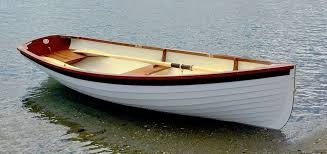
\includegraphics[width=\linewidth]{../Images/boat.jpg}
		\caption{A Boat.}
		\label{fig:boat1}
	\end{figure}
	
	Figure \ref{fig:boat1} shows a boat.
		
	% Example 1:
	\ldots when Einstein introduced his formula
	\begin{equation}
		e = m \cdot c^2 \; ,
	\end{equation}
	which is at the same time the most widely known and the least
	well understood physical formula
	
	% Example 2:
	\ldots from which follows Kirchoff's current law:
	\begin{equation}
		\sum_{k=1}^{n} I_k = 0 \; ,
	\end{equation}
	Kirchoff's voltage law can be derived \ldots
	
	% Example 3:
	\ldots which has several advantages.
	\begin{equation}
		I_D = I_F - I_R
	\end{equation}
	is the core of a very different transistor model. \ldots
	
	\begin{equation}
		f(x) = x^2
	\end {equation}
	
	\begin{equation*}
		3+ 3 = 6
	\end {equation*}
	\begin{equation*}
		1 = 5 - 4
	\end {equation*}
	
	\begin{align*}
	% The ampersand identifies where the equations will align
		1 &= 5 - 4\\ % In this case the \\ indicates a new line
		3+ 3 &= 6\\ 
		\\
		f(x) &= x^2\\
  		g(x) &= \frac{1}{x}\\
  		F(x) &= \int^a_b \frac{1}{3}x^3
	\end {align*}